\documentclass[a4paper, 12pt]{article}

\usepackage[T2A]{fontenc}
\usepackage[utf8]{inputenc}
\usepackage[english,russian]{babel}
\usepackage[left=15mm, top=20mm, right=15mm, bottom=20mm, nohead, nofoot]{geometry}

\usepackage{hyperref}

\usepackage{wrapfig}
\usepackage{afterpage}
\usepackage{amsmath, amsfonts, amssymb, amsthm, mathtools}
\author{}
\title{}
\date{}
%%%%%%%%%%%%%%%%%%%%%%%%%%%%%%%%%%%%%%%%%%%%%%%%%%%%%%%%%%%%%%%%%%%%%%%%%
\usepackage{fancyhdr}
\usepackage{lastpage}
\usepackage{graphicx, wrapfig, subcaption, setspace, booktabs}
\usepackage[T1]{fontenc}
\usepackage[font=small, labelfont=bf]{caption}
\usepackage[protrusion=true, expansion=true]{microtype}
\usepackage[english]{babel}
\usepackage{sectsty}
\usepackage{url, lipsum}
\newcommand{\HRule}[1]{\rule{\linewidth}{#1}}
\onehalfspacing
\setcounter{tocdepth}{5}
\setcounter{secnumdepth}{5}

\usepackage{graphicx}
\graphicspath{{pictures/}}
\DeclareGraphicsExtensions{.pdf,.png,.jpg}
\usepackage{multirow}

\usepackage[autoplay, loop, nomouse, controls]{ animate}
\usepackage[autoplay, repeat]{ movie 15}
%%%%%%%%%%%%%%%%%%%%%%%%%%%%%%%%%%%%%%%%%%%%%%%%%%%%%%%%%%%%%%%%%%%%%%%%%


\begin{document}

\title{ \normalsize \textsc{ВОПРОС ПО ВЫБОРУ}
		\\ [4.0cm]
		\HRule{0.5pt} \\ [0.3cm]
		\LARGE \textbf{{БРАХИСТОХРОНА}}
		\HRule{0.5pt} \\ [0.1cm]
		\normalsize  \vspace*{20\baselineskip}}

\date{}

\author{
		Маллаев Руслан, Б02-005 \\
ЛФИ, 2020\\ }

\maketitle
\thispagestyle{empty}
\newpage
\part{Введение}

$\huge{\text{В}}$ 1996-ом году Иоганн Бернулли опубликовал статью, в которой поставил следующую задачу:

\begin{quote}
\begin{large}
Среди плоских кривых, соединяющих две данные точки A и B, лежащих в одной вертикальной плоскости (B ниже A), найти ту, двигаясь по которой под действием только силы тяжести, сонаправленной отрицательной полуоси OY, материальная точка из A достигнет B за кратчайшее время.
\end{large}
\end{quote}

На статью Иоганна Бернулли откликнулись Исаак Ньютон, Якоб Бернулли, Г. В. Лейбниц, Г. Ф. Лопиталь, Э. В. Чирнхаус. Все они, как и сам Иоганн Бернулли решили задачу разными способами. Метод решения, полученного 26 января 1697 года Исааком Ньютоном, лёг в основу важнейшей области естествознания — вариационного исчисления.

\begin{center}
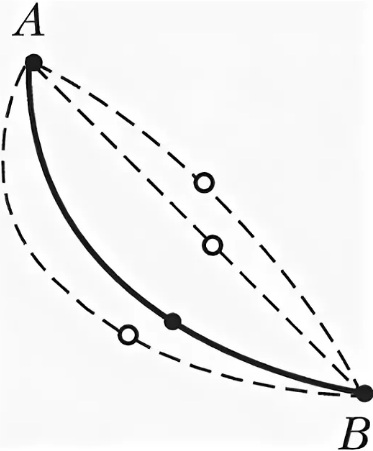
\includegraphics[scale=0.5]{brah}
\end{center}
\[\textit{Брахистохрона}\]

%\begin{center}
%\includemovie[autoplay , repeat]{8cm}{8cm}{brachistochrone.avi}
%\end{center}
\newpage


\part{Решение Исаака Ньютона}

Пусть имеются две произвольные точки, расположенные на разных ординатах. Далее пусть произвольная материальная точка M скатывается от точки A к точке B под действием только силы тяжести (силы трения отсутствуют). Найдём такую траекторию, при которой время скатывания будет минимально.

Направим ось ординат вниз и сопоставим начальной точке нулевое значение ординаты. Запишем закон сохранения энергии для материальной точки M: 
\[\frac{mv^2}{2} = mgy,\]
где\\
    m — масса тела,\\
    g — ускорение свободного падения,\\
    y — ордината,\\
    v — скорость движения тела.\\
Получаем:
\[v = \sqrt{2gy},\]
откуда можно найти значение проекции скорости на ось x:
\[v_x = \frac{v}{\sqrt{1 + (y')^2}} = \frac{\sqrt{2gy}}{\sqrt{1 + (y')^2}}\] 
Поскольку время на спуск равняется $\displaystyle \int\limits_a^b \frac{1}{v_x}dx$, то задача сводится к минимизации значения интеграла
\[\frac{1}{\sqrt{2g}}\displaystyle \int\limits_a^b \frac{\sqrt{1 + (y')^2}}{\sqrt{y}}dx\]
\newpage

\part{Решение Якоба Бернулли}
Решение Я. Бернулли выделялось из всех представленных как своей нетривиальностью, так и общностью применяемых методов. Первым принципом, из которого исходил Я. Бернулли при решении, был тот, что если кривая имеет какое-либо свойство, то тем же свойством должна обладать и любая её часть. Эта идея позволила разбить одну сложную задачу на несколько более простых. Второй принцип — весьма оригинальная идея применения законов оптики в механике.

Закон оптики, о котором идёт речь, называют принципом Ферма:

\begin{quote}
\begin{large}
Из всех возможных путей свет выбирает тот путь, на который требуется наименьшее время.
\end{large}
\end{quote}

Из этого одного единственного постулата вытекают все законы геометрической оптики, в частности, закон преломления света на границе двух сред, открытый голландцем В. Снеллом (van Snel van Royen) в 1621 году.
\begin{center}
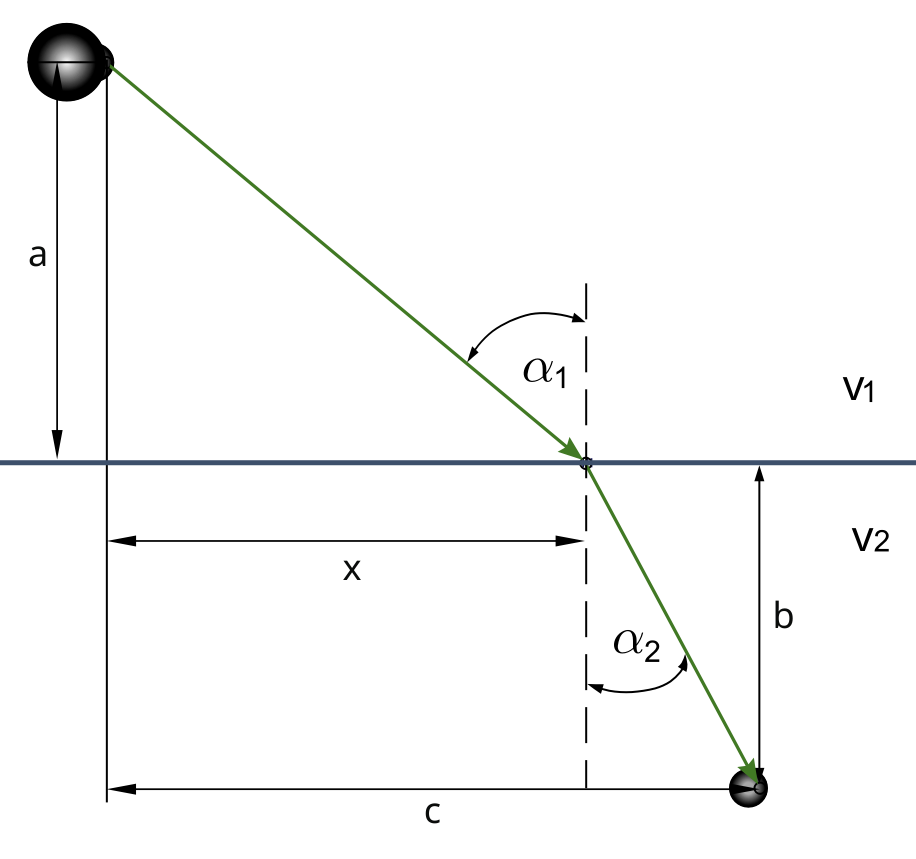
\includegraphics[scale=0.5]{snell}
\end{center}
\[\textit{К закону Снелла}\]

Луч света из среды, в которой он имел скорость $v_1$, попадает в среду, где его скорость равна $v_2$. Найдём, применяя принцип Ферма, как связаны величины $v_1$, $v_2$ и $\alpha_1$, $\alpha_2$ (см. рис). Время, необходимое для прохождения луча света от точки A до точки B, равно 
\[T(x) = \frac{\sqrt{a^2 + x^2}}{v_1} + \frac{\sqrt{b^2 + (c - x)^2}}{v_2}.\]
В соответствии с принципом Ферма нужно найти минимум функции T(x), для чего требуется решить уравнение 
\[\frac{dT}{dx} = 0,\]
откуда получим
\[\frac{x}{v_1\sqrt{a^2 + x^2}} = \frac{c - x}{v_1\sqrt{b^2 + (c + x)^2}},\]
или, что то же самое,
\[\frac{\sin\alpha_1}{v_1} = \frac{\sin\alpha_2}{v_2}\]

Обращаясь непосредственно к решению задачи, разобъём область, в которой лежит путь катящейся точки, на n полос ширины h (см. рис) и предположим, что скорость точки меняется скачками на границах полос, оставаясь постоянной внутри каждой области разбиения. Тогда скорость будет последовательно принимать следующие значения: $v_n = \sqrt{2gnh}, v_{n-1} = \sqrt{2g(n-1)h}, v_1 = \sqrt{2gh}$, а точка двигаться по ломаной линии. При этом чем больше число n разбиений (и, соответственно, меньше величина h) будет браться, тем менее построенная ломаная линия будет отличаться от искомой кривой. 
\begin{center}
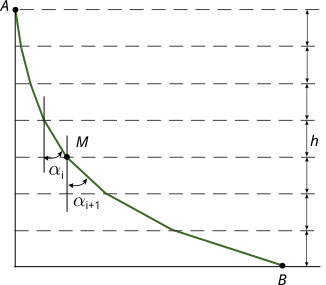
\includegraphics[scale=1.5]{brahistohrona}
\end{center}
\[\textit{К решению задачи о брахистохроне}\]
Вспоминая закон Снелла и применяя его к материальной точке, получим 
\[\frac{\sin\alpha_i}{\sin\alpha_{i+1}} = \frac{\sqrt{2gih}}{\sqrt{2g(i+1)h}},\]
где i=1,2,…,n. Таким образом, имеем 
\[\frac{\sin\alpha_1}{\sqrt{h}} = \frac{\sin\alpha_2}{\sqrt{2h}} = ... = \frac{\sin\alpha_n}{\sqrt{nh}}\]
т. е. отношение синуса угла между любым звеном ломаной и вертикалью к корню квадратному из расстояния соотвествующего слоя от верхней линии разбиения есть величина постоянная. В пределе при $n \longrightarrow \infty$ направление каждого звена ломаной перейдёт в касательную к искомой кривой, для которой будет, следовательно выполняться соотношение
\begin{equation}
\sin\alpha = c\sqrt{y},
\end{equation}
где c — коэффициент пропорциональности, $\alpha$ — угол между касательной к кривой и вертикалью. Последнее условие однозначно определяет кривую, известную как циклоида. Таким образом, кривая наискорейшего спуска является циклоидой.

Нам осталось показать, что соотношение (1) необходимо и достаточно для того, чтобы кривая, ему удовлетворяющая, была циклоидой. Циклоида представляет собой траекторию, описываемую точкой окружности, катящейся без скольжения по прямой линии. Для удобства обозначим угол между касательной к циклоиде и вертикалью через $\beta / 2$, угол наклона касательной к горизонтали — $\gamma$, радиус «производящей» окружности обозначим r (см. рис).
\begin{center}
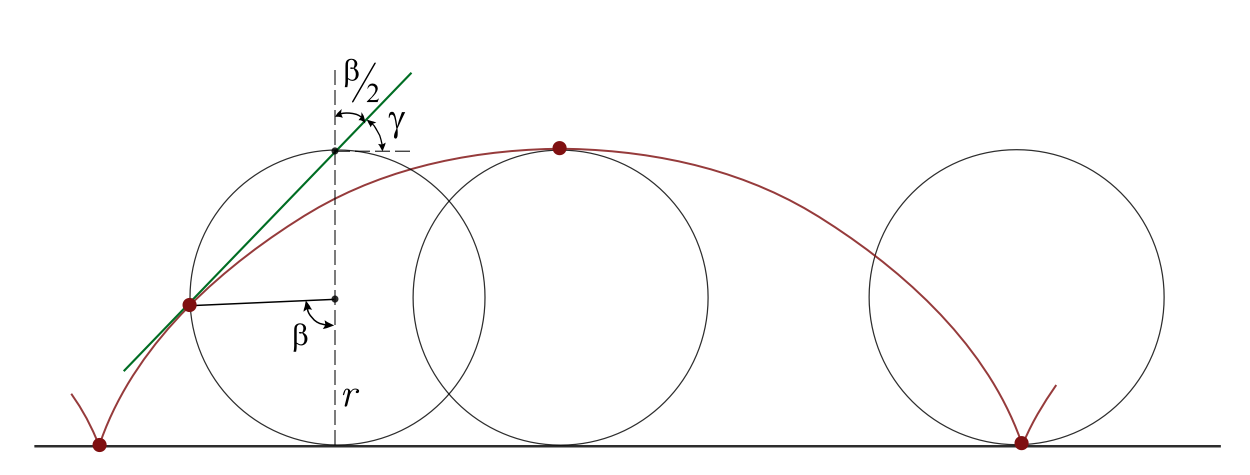
\includegraphics[scale=0.5]{cycloida}
\end{center}
\[\textit{Циклоида}\]
Тогда уравнение циклоиды в полярных координатах будет иметь вид
\begin{equation}
x = r(\varphi - \sin\varphi),\text{ }\text{ }\text{ } y = r(1 - \cos\varphi),
\end{equation}

Распишем $\sin\alpha$ из уравнения (1):
\[\sin\alpha = \frac{1}{\sqrt{1 - (y')^2}},\]
из уравнения циклоиды (2)
\[y'_x = \frac{dy}{dx} = \frac{dy}{d\varphi}\frac{d\varphi}{dx} = \frac{r\sin\varphi d\varphi}{r(1 - \cos\varphi)d\varphi} = \frac{\sin\varphi}{1 - \cos\varphi},\]
откуда
\[\sin\alpha = \frac{\frac{1 - \cos\varphi}{2}}{\sqrt{\frac{1 - \cos\varphi}{2}}} = \sqrt{\frac{1 - \cos\varphi}{2}} = \sin\frac{\varphi}{2},\]
тогда $\sin\frac{\varphi}{2}$ выразим из зависимости $y(\varphi)$ системы уравнений (2)
\[\sin\frac{\varphi}{2} = \frac{1}{\sqrt{2r}} \sqrt{y},\]
а условие (1) перепишется так: \\
\begin{equation}
\sin\alpha = \sin\frac{\varphi}{2} = \frac{1}{\sqrt{2r}} \sqrt{y} .
\end{equation}
Поскольку $1 - \cos\beta = 2\sin^2 (\beta /2)$, из уравнения (2) сразу следует условие (3). Обратно, имеем 
\[\gamma = \frac{\pi}{2} - \frac{\varphi}{2}, \text{ }\text{ }\text{ } \tg\gamma = \ctg\frac{\varphi}{2}.\]
Следовательно, 
\[\frac{dy}{dx} = \ctg\frac{\varphi}{2},\]
откуда 
\[\frac{d\varphi}{dx}\frac{dy}{d\varphi} = \ctg\frac{\varphi}{2}, \text{ }\text{ }\text{ }\frac{d\varphi}{dx}r\sin\varphi = \ctg\frac{\varphi}{2}\]
и, после несложных преобразований, имеем простое дифференциальное уравнение 
\[\frac{dx}{d\varphi} = r(1 - \cos\varphi)\]
решение которого с учётом начального условия x(0)=0, совпадает с первым уравнением из системы (2), задающей циклоиду. 
\newpage

\part{Таутохрона}
А что, если существует кривая, скатываясь с любой точки которой(под действием силы тяжести) тело будет достигать конечную точку за фиксированный промежуток времени(то есть время спуска не будет зависеть от начального положения)? Первым эту кривую идентифицировал Христиан Гюйгенс в 1659-ом году(на 38 лет раньше нахождения кривой брахистохроны Иоганном Бернулли). Он показал, что данной кривой является циклоида.

К примеру, если запустить маятники с разными амплитудами совершать колебания по циклоиде, то периоды колебания таких маятников будут одинаковыми
\begin{center}
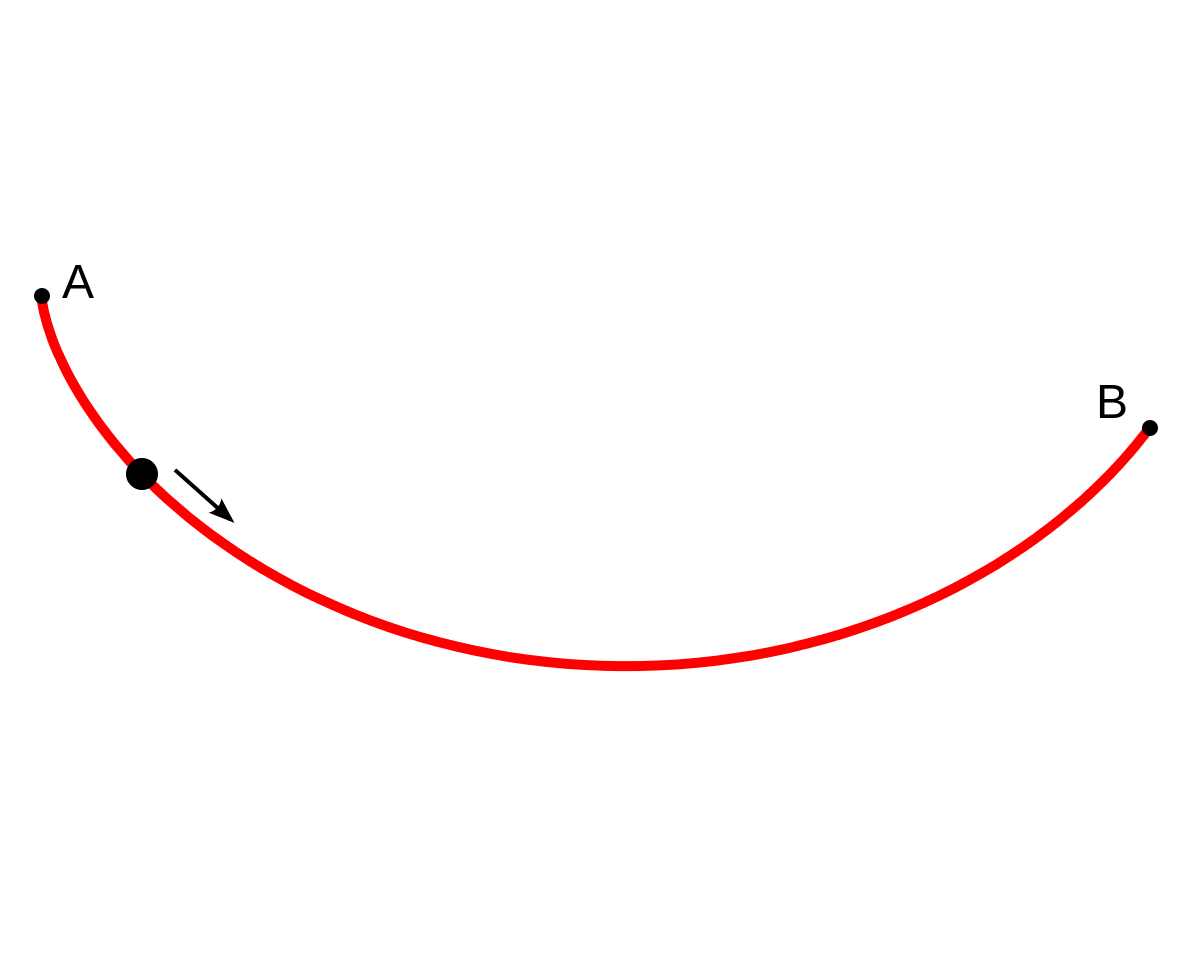
\includegraphics[scale=0.2]{taut}
\end{center}
\[\textit{Таутохрона}\]

%\begin{center}
%\animategraphics[width =0.4\linewidth ,autoplay, loop, nomouse]{60}{220px-%Isochronous_cycloidal_pendula}{}{}
%\end{center}
%\[\textit{Пять изохронных циклоидальных маятников с разными амплитудами}\]

Не будем описывать процесс решения задачи нахождения кривой таутохроны, а лишь докажем, что циклоида удовлетворяет условию таутохроны.

Уравнение циклоиды в декартовой системе координат имеет вид
\[x = r\arccos\frac{r-y}{r} - \sqrt{2ry - y^2},\]
\begin{center}
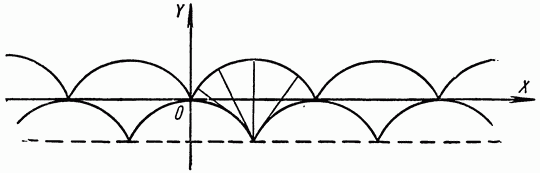
\includegraphics[scale=1.3]{arch}
\end{center}
\[\textit{Циклоида}\]
по теореме о производной обратной функции имеем
\[y'_x = \frac{1}{x'_y},\]
из уравнения циклоиды получим производную x по y:
\[x'_y = \frac{y}{\sqrt{2ry - y^2}},\]
то есть
\[y'_x = \sqrt{2\frac{r}{y} - 1}.\]

Скорость точки при движении в поле силы тяжести зависит только от разности начальной и конечной координат по оси Y(ось направлена вниз):
\[|v| = \sqrt{2g(y - y_0)},\]
проекция скорости на ось Y, соответсвенно
\[v_y = \frac{y'}{\sqrt{1 + (y')^2}}\cdot\sqrt{2g(y - y_0)},\]
подставив ранее выраженную производную y', а также упростив выражение получим
\[v_y = \sqrt{1 - \frac{y}{2r}}\cdot\sqrt{2g(y - y_0)}.\]

Теперь выразим время спуска точки до ординаты, при которой y' = 0, то есть y = 2r
\[\displaystyle\int\limits_0^\tau dt = \int\limits_{y_0}^{2r} \frac{dy}{v_y} = \frac{1}{\sqrt{g}}\int\limits_{y_0}^{2r} \frac{dy}{\sqrt{1 - \frac{y}{2r}}\cdot\sqrt{2(y - y_0)}} = \frac{\sqrt{r}}{\sqrt{g}}\int\limits_{y_0}^{2r} \frac{dy}{\sqrt{-y^2 + y(2r + y_0) - 2ry_0}},\]
откуда
\[\tau = -\frac{\sqrt{r}}{\sqrt{g}}\frac{2\sqrt{(2r - y_0)(y_0 - y)}\cdot\sqrt{\frac{y - 2r}{y_0 - 2r}}\cdot\ln (\sqrt{\frac{y_0-y}{2r - y_0}+1} + \sqrt{\frac{y_0 - y}{2r - y_0}})}{\sqrt{(y_0 - y)(y - 2r)}}\Bigg|_{y_o}^{2r},\]
\[\tau = -2i\frac{\sqrt{r}}{\sqrt{g}}\ln (\sqrt{\frac{y_0-y}{2r - y_0}+1} + \sqrt{\frac{y_0 - y}{2r - y_0}}); (y = 2r),\]
\[\tau = -2i^2\frac{\sqrt{r}}{\sqrt{g}} \cdot \frac{\pi}{2} = \pi\frac{\sqrt{r}}{\sqrt{g}}.\]

Таким образом, доказано, что при спуске по циклоиде время скатывания до самой нижней точки не зависит от начальной координаты скатываемой точки на циклоиде(понятно, что начальная точка должна находиться выше конечной).


\newpage

\part{Использование брахистохроны}
Кривую брахистохрону используют инженеры, например, проектировщики американских горок. У них есть потребность разогнать машину до максимально возможной скорости при максимально коротком вертикальном падении.
\begin{center}
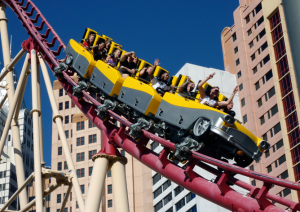
\includegraphics[scale=1]{горки}
\end{center}
\[\textit{Американские горки}\]

Также можно найти использование свойств брахистохроны в спорте. Горнолыжникам, к примеру, требуется достигнуть определенной точки не по наикратчайшему пути, а по пути, который приведет их к финишу быстрее всего.



\end{document}
